\chapter{Piattaforma di Simulazione}\label{chap:sim}

La piattaforma di simulazione è uno strumento di fondamentale importanza al fine di validare l'infrastruttura software proposta. È inoltre un valido strumento per valutare l'impatto dell'introduzione della mobilità elettrica veicolare all'interno di un determinato contesto. Grazie ad esso si può prevedere il numero di veicoli che la grid potrà supportare, quante colonnine saranno necessarie e che potenza dovranno avere. Risulta quindi uno strumento fondamentale sia dal punto di vista dell'amministrazione pubblica/cittadina, per prevedere un piano urbanistico sostenibile, che dal punto di vista dei gestori della rete elettrica, i quali potranno valutare la richiesta energetica di tale scenario ed eventualmente prevedere investimenti in quella direzione.

\section{Architettura}

Per simulare gli innumerevoli aspetti legati all'Electrical Mobility sono stati usati diversi simulatori/tecnologie in simbiosi. In questa sezione verranno analizzate sommariamente per introdurre il resto della trattazione.

\subsection{SUMO}\label{sebsec:sumo}

SUMO (Simulator of Urban Mobility) è un simulatore Open Source e multi-piattaforma di traffico urbano progettato per simulare reti stradali di grandi dimensioni. Sviluppato in C++ è supportato principalmente dall'Institute of Transportation Systems at the German Aerospace Center. La simulazione è di tipo microscopico ovvero ogni veicolo è modellato in modo esplicito, ha un proprio itinerario e si muove individualmente attraverso la rete. Ogni aspetto relativo alla simulazione viene configurato attraverso file XML di descrizione della rete stradale, dei parametri e percorsi di ogni singolo veicolo ed eventualmente di altri aspetti legati alla simulazione come i flussi di traffico e la descrizione degli edifici. 

SUMO permette di avviare la simulazione in due modalità:

\begin{itemize}
	\item \textbf{Visuale}: rende disponibile un riscontro visuale dell'andamento della simulazione tramite un interfaccia che mostra la mappa della rete/città con vista dall'alto. Vengono mostrati tutti i veicoli ed è possibile accedere a tutti i parametri della simulazione. Vengono mostrati inoltre i semafori agli incroci, la segnaletica delle strade e, nel caso siano stati caricati, gli edifici della città. Tutto questo ovviamente impatta notevolmente sulle performance ma, al di la del gradevole ed efficace effetto visivo, è utile per monitorare come evolve la simulazione. L'abbiamo usato ad esempio per assicurarsi che i veicoli si fermassero alle colonnine, oppure per valutare la quantità di traffico generata in seguito all'inserimento di un determinato numero di veicoli. È stato molto utile è anche in fase di Demo per mostrare il funzionamento del simulatore.
	\item \textbf{Testuale}: vengono stampati nel terminale i messaggi di Warning ed Error e opzionalmente qualche messaggio integrativo di debug per indicare gli step di avanzamento della simulazione. Una volta constatato, tramite la modalità visuale, che la simulazione si comporta come previsto si passa a questa modalità che offre performance maggiori. È quindi particolarmente indicata per le simulazioni di lunga durata.
\end{itemize}

\subsubsection{Tools}\label{sumo-tools}

I file XML che descrivono le simulazioni possono diventare molto complessi qualora si decida di simulare scenari realistici (come Bologna). SUMO rende disponibili innumerevoli tool automatici per la generazione dei file di configurazione. In questa tesi prenderò in esame solo quelli che si sono rivelati utili:

\begin{itemize}
 	\item \textbf{netconvert}: genera file con estensione .net.xml di mappatura della rete stradale. La generazione avviene in modo pseudo-casuale, tramite la definizione dei nodi e degli archi che definiscono il grafo della rete stradale oppure, come nel nostro caso, attraverso la conversione da formati esterni(OpenStreetMap, VISUM, VISSIM, OpenDRIVE, MATsim ecc..)
 	\item \textbf{polyconvert}: Genera file con estensione .poly.xml contenenti le informazioni relative agli edifici, zone di verde, fiumi laghi ecc.. Anch'esse vengono importate dai file delle mappe in altri formati.
 	 \item \textbf{duarouter}: Genera file con estensione .rou.xml descrittivi del percorso di ogni veicolo, compresi tutti gli step intermedi. La generazione dei percorsi avviene applicando un algoritmo di cammino su grafi a scelta tra \emph{Dijikstra} o \emph{A*}. I punti di partenza e arrivo vengono generati casualmente da uno script in python reso disponibile tra i tool di SUMO (\code{randomTrips.py}).
\end{itemize}

\subsubsection{TRaCI}

TraCI (Traffic Controller Interface) è un modulo, reso disponibile da SUMO, che permette di interagire con la simulazione in tempo reale tramite un protocollo Client/Server basato su TCP/IP. All'avvio della simulazione SUMO si mette in ascolto su una porta in attesa di messaggi. Qualunque linguaggio che supporti il protocollo TCP/IP può dunque modificare lo stato della simulazione oppure ricevere notifiche sul cambiamento di variabili alle quali ci si può sottoscrivere. È proprio TraCI che farà da ponte tra SUMO e l'altro simulatore usato all'interno della nostra piattaforma.

\subsection{OMNeT++}

OMNeT++ è un ambiente OpenSource di simulazione a eventi discreti. È principalmente usato per la simulazione di reti di comunicazione ma, grazie alla sua architettura modulare ed estremamente flessibile, è possibile utilizzarlo negli ambiti più disparati come la simulazione di sistemi informatici complessi, architetture hardware o, come nel nostro caso, per supporto alla simulazione veicolare.

Le simulazioni vengono modellate tramite l'impiego di componenti riusabili chiamati \emph{moduli} combinabili tra di loro come blocchi LEGO.

I moduli possono essere connessi tra di loro attraverso i \emph{gates} e combinati insieme per formare dei moduli composti (compound modules). La comunicazione tra moduli normalmente avviene tramite message passing e i messaggi possono contenere strutture dati arbitrarie (assieme informazioni predefinite tipo i \emph{timestamp}). Questi messaggi possono viaggiare attraverso percorsi predefiniti dai \emph{gates} e dalle \emph{connections} oppure essere inviati direttamente alla loro destinazione, scelta molto utile nel caso delle comunicazioni wireless. 

I moduli, i relativi parametri e i collegamenti fra di essi vengono definiti tramite un linguaggio di alto livello (NED) in appositi file con estensione .ned, mentre la logica viene implementata in una corrispondente classe C++.

OMNeT++ viene distribuito con un IDE basato su Eclipse grazie al quale si possono eseguire molteplici operazioni in modo visuale, come ad esempio la creazione e aggregazione di moduli.

Anche OMNeT++ mette a disposizione due modalità di esecuzione della simulazione: una visuale (\emph{Tkenv}) e una testuale (\emph{Cmdenv}). La modalità visuale che permette di vedere i moduli con i relativi messaggi scambiati viene usata in fase di debug o in fase di Demo. La modalità testuale, ovviamente più performante e adatta alle simulazioni batch, mostra solo i messaggi di debug della simulazione insieme allo \emph{standard output} dei moduli. Per i nostri scopi abbiamo usato solo la modalità testuale.

Un punto di forza di OMNeT++ è costituito dagli strumenti resi disponibili per l'analisi dei dati generati dalle simulazioni. Questo permette di applicare in tempo reale trasformazioni e aggregazioni tra i set di dati e infine di visualizzare i risultati con varie tipologie di grafici: a barre, a linee, istogrammi ecc\dots

In OMNeT++ si possono registrare due tipi di dato: i vettori e gli scalari. Nel caso dei vettori i dati sono rappresentati nel piano cartesiano con il tempo come ascissa e il dato come ordinata. Nel caso degli scalari si registra solamente il dato.

\subsection{Veins}\label{subsec:veins}

Veins è un framework OpenSource per la simulazione di reti veicolari IVC (Inter-Vehicular Communication). Utilizza OMNeT++ e SUMO in simbiosi. Si appoggia su MiXiM, un framework per OMNeT++ che implementa modelli per reti wireless fisse e mobili (reti di sensori wireless, reti ad hoc, reti veicolari ecc\dots). La comunicazione con SUMO avviene tramite TRaCI. Ogni volta che nella simulazione in SUMO viene aggiunto un veicolo, Veins crea dinamicamente un corrispondente modulo OMNeT++ che permette di controllarlo sotto ogni aspetto (percorso, colore, velocità, accelerazione, parcheggio ecc..).

Il simulatore consiste in un modulo di Veins opportunamente modificato per disporre di un ambiente contenente solo i componenti indispensabili allo scopo. Le performance sono infatti determinanti per ottenere risultati in tempi utili. Infatti sono stati rimossi da Veins i moduli necessari alla comunicazione wireless (nic80211 e ARP) e il modulo per la gestione degli ostacoli (obstacles) che era utilizzato per la gestione dello shadowing delle reti wireless.

\subsubsection{Il funzionamento di Veins}\label{subsubsec:veins-func}

Veins è il ponte tra OMNeT++ e SUMO e la comunicazione tra i due avviene tramite TraCI. In realtà ``in mezzo'' ai due simulatori si trova uno script python, \emph{sumo-launchd.py}, in ascolto sulla prima porta libera che trova, in attesa che venga avviato Veins. Veins appena avviato si connette a questo script che a sua volta lancia SUMO. A questo punto inizia la sincronizzazione tra i due simulatori che avviene tramite ``staffetta'' come mostrato in Fig. ~\ref{fig:veins-state-machine}. Per garantire l'esecuzione sincrona a intervalli definiti Veins inserisce in un buffer tutti i comandi da inviare a SUMO (Fig.  ~\ref{fig:veins-sequence-diagram}). Ad ogni passo temporale i comandi contenuti nel buffer vengono inviati. Questo innesca l'avanzamento del corrispondente passo temporale nella simulazione del traffico stradale. Al termine dello step temporale di simulazione del traffico stradale, SUMO invia in risposta a Veins una serie di comandi con lo stato e la posizione di tutti i veicoli istanziati. Dopo l'elaborazione di tutti i comandi ricevuti, Veins aggiunge i corrispettivi nodi per ogni nuovo veicolo introdotto nella simulazione e rimuove i nodi relativi ai veicoli giunti a destinazione. A questo punto la simulazione può avanzare al prossimo step temporale.

\begin{figure}[H]
        \centering
        \begin{subfigure}[H]{0.5\textwidth}
                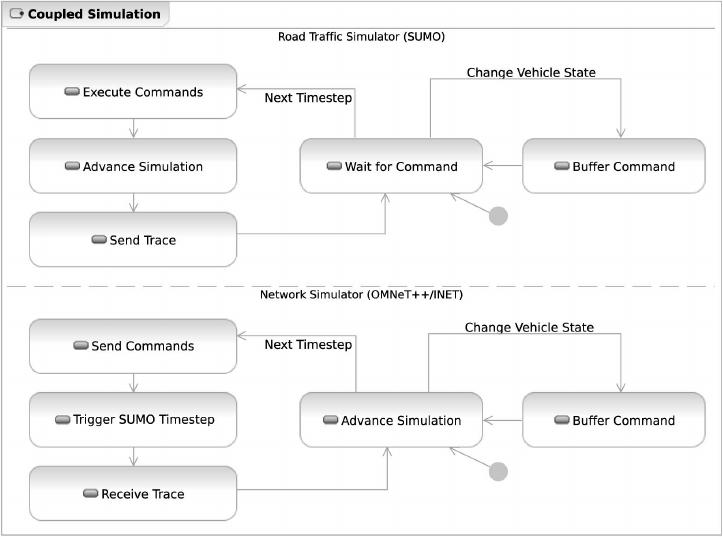
\includegraphics[width=\textwidth]{assets/veins-state-machine.jpg}
                \caption{Panoramica dei due simulatori abbinati. Macchina a stati di SUMO e i moduli di Veins.}
                \label{fig:veins-state-machine}
        \end{subfigure}%
        ~ %add desired spacing between images, e. g. ~, \quad, \qquad etc.
          %(or a blank line to force the subfigure onto a new line)
        \begin{subfigure}[H]{0.5\textwidth}
                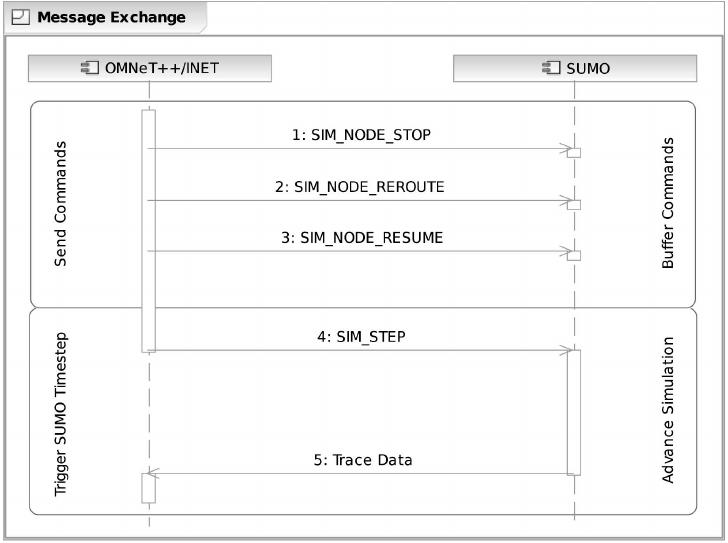
\includegraphics[width=\textwidth]{assets/veins-sequence-diagram.jpg}
                \caption{ Diagramma di sequenza dei messaggi scambiati tra SUMO e Veins. L'esecuzione dei comandi è ritardata fino al successivo passo temporale in SUMO.}
                \label{fig:veins-sequence-diagram}
        \end{subfigure}
        \caption{Architettura Veins}
\end{figure}


\section{Modellazione della Simulazione}

L'intera simulazione viene incapsulata all'interno di una Network. Il Network è lo scenario da simulare al cui interno si definiscono i moduli che compongono la simulazione. Come mostrato in Fig \ref{fig:module-scenario} sono sostanzialmente quattro i moduli che compongono la nostra simulazione:

\begin{itemize}
	\item \textbf{world}: è un modulo di tipo \code{BaseWorldUtility}, fornito da MiXiM, che rappresenta l'area di circoscrizione dello scenario simulato. Come parametri di ingresso richiede la definizione della grandezza dello scenario in metri. La mappa usata in SUMO non può essere più grande delle dimensioni definite in questo modulo.
	\item \textbf{traciManager}: è un modulo di tipo \code{TraCIScenarioManagerLaunchd}, fornito da Veins, che mette in comunicazione OMNeT++ con SUMO. Tutti i messaggi inviati a TraCI passano da questo modulo (l'implementazione vera e propria della comunicazione con TraCI avviene nel modulo padre \code{TraCIScenarioManager}), fondamentale in quanto crea un modulo OMNeT++ per ogni veicolo di SUMO.
	\item \textbf{cityService}: rappresenta la grid. Contiene infatti i GCP e gli EVSE. Ricopre anche la funzione di raccoglitore delle statistiche globali su colonnine e veicoli (Sez: \ref{sec:module-city}).
	\item \textbf{connectionManager}: si occupa della comunicazione tra moduli ma è inutilizzato. Non l'ho rimosso per garantire la compatibilità con Veins.
\end{itemize}

Ogni volta che SUMO crea un veicolo, Veins provvede a creare il corrispondente modulo \code{Car} in OMNeT++ (Fig. \ref{fig:module-car}).  \code{Car} in realtà è un modulo composto, ovvero un contenitore, privo di implementazione che contiene altri moduli. Di default conterrebbe tutti i componenti relativi alle comunicazioni wireless in quanto sarebbe il target di Veins, ma li ho rimossi in quanto non utili, per ora, nello scenario attualmente simulato.

Per rendere la simulazione il più possibile attinente alla realtà risulta necessario implementare i modelli di carica e scarica dei veicoli e i modelli comportamentali degli utenti oltre l'implementazione dei moduli di comunicazione con il servizio cittadino. Per svolgere questi compiti è stato necessario arricchire la definizione di Car con 3 nuovi moduli:

\begin{itemize}
	\item \textbf{TraciMobility}: è un modulo fornito da Veins che mette in comunicazione il veicolo con SUMO tramite TRacI.
	\item \textbf{CarLogic}: il modulo principale in cui è implementata la logica del veicolo. 
	\item \textbf{Battery}: implementa il modello di carica e scarica del veicolo.
	\item \textbf{DriverBehaviour}: implementa i comportamenti che l'utente assume in occasione a determinate scelte.  
\end{itemize}

Ogni modulo contiene parametri che permettono di cambiarne il comportamento. Grazie a OMNeT++ diventa semplice lanciare molteplici simulazioni con diversi set di dati. Particolarmente interessante è la possibilità di eseguire la simulazione senza prenotazione per confrontare le differenze di occupazione delle colonnine rispetto allo scenario con prenotazione.

\begin{figure}
        \centering
		\begin{subfigure}[H]{0.45\textwidth}
                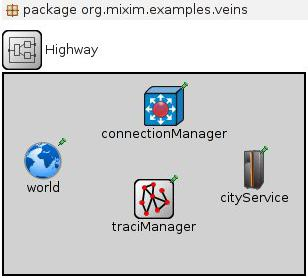
\includegraphics[width=\textwidth]{assets/module-scenario.jpg}
                \caption{Modulo scenario}
                \label{fig:module-car}
        \end{subfigure}
        \qquad
        \begin{subfigure}[H]{0.45\textwidth}
                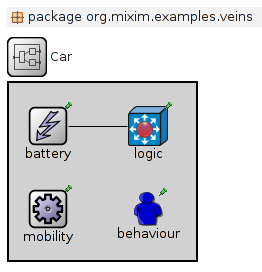
\includegraphics[width=\textwidth]{assets/module-car.png}
                \caption{Modulo Car}
                \label{fig:module-scenario}
        \end{subfigure}%
        \caption{Moduli OMNeT++}
\end{figure}

\subsection{Ciclo di Vita dei moduli}\label{subsec:lifecycle}

Essendo OMNeT++ un simulatore a eventi discreti, i moduli in esso implementati non fanno nulla finché non viene schedulato un evento. Gli eventi vengono schedulati attraverso messaggi inviati dai moduli stessi. Sostanzialmente si tratta di decidere quando, a chi e cosa mandare.

\emph{Chi} è il modulo destinatario del messaggio, come vedremo più avanti può coincidere con il mittente.

\emph{Quando} è l'istante di simulazione in cui il messaggio verrà ricevuto dal modulo destinatario. In quanto tale deve essere schedulato nel futuro o tuttalpiù nell'istante corrente di simulazione.

\emph{Cosa} è il messaggio da inviare. OMNeT++ fornisce un un messaggio di base, \code{cSimpleMessage}, ma, come vedremo più avanti, è possibile definirsi messaggi propri più complessi.

All'interno di questa simulazione non c'è uno scambio di messaggi tra i diversi moduli, per cui risulta necessario auto-inviarsi i messaggi per mantenere \emph{vivo} il modulo.

Quando Veins crea un modulo il corrispondente veicolo in SUMO viene aggiornato ogni 0.1 secondi, step temporale di default. In OMNeT++, invece, è il programmatore a decidere ogni quanto tempo aggiornare un modulo mediante il meccanismo degli auto-messaggi. Schedulando i messaggi in modo intelligente si può guadagnare in performance poiché ci si può inviare il messaggio solo quando è realmente necessario.

Quando un modulo \code{Car} viene creato, OMNeT++ invoca la funzione \code{initialize()} di cui il programmatore può eseguire l'override e nella quale, dopo le opportune inizializzazioni, è necessario auto-schedularsi un messaggio. I messaggi vengono ricevuti dalla funzione \code{handleMessage()}. Dall'interno di questa funzione si può implementare la logica del modulo che continua a \emph{vivere} finché il corrispondente veicolo in SUMO giunge a destinazione. In questo istante Veins, tramite la classe \code{TraCIScenarioManager}, rileva che il veicolo è uscito dalla simulazione e quindi lo elimina anche da OMNeT++ che invoca la funzione di terminazione \code{finish()}.

\subsection{CityService}\label{sec:module-city}

Il modulo simula la grid e al suo avvio carica le informazioni relative ai GCP presenti nello scenario simulato da un file XML. Il file utilizzato è lo stesso del servizio cittadino (Sez. ~\ref{subsubsec:city-init}). Le colonnine caricate vengono trasformate in oggetti C++ fruibili dai veicoli virtuali.

Per chiarezza è necessario distinguere tra il modulo  \code{CityService} di OMNeT++ e il CS visto in precedenza. Nel seguito mi riferirò al primo con il nome intero e al secondo con l'abbreviazione.

Mediante il settaggio di parametri esterni, \code{CityService}, abilita/disabilita le prenotazioni, e decide il tasso di penetrazione di veicoli elettrici nello scenario.

Di seguito i parametri del modulo:

\begin{itemize}
	\item \code{gcpList}: percorso del file XML contenente la definizione dei GCP. Deve essere lo stesso utilizzato dal servizio cittadino reale.
	\item \code{electricalVehicleFreq}: stabilisce la frequenza di immissione di veicoli elettrici nella simulazione. Variabile da 0 a 100 indica la probabilità che il veicolo immesso nella simulazione sia elettrico. Occorre ricordare che il numero e la frequenza con cui i veicoli vengono immessi nella simulazione è determinato dai file di configurazione di SUMO. 
	\item \code{maxElectricalVeh}: impone un limite superiore al numero di veicoli che possono essere presenti nella simulazione in un determinato istante. Questo significa che, raggiunto il massimo numero di veicoli, e uno di essi lascia la simulazione per qualunque motivo, allora verrà sostituito da uno nuovo, ammesso che SUMO generi altri veicoli e che la statistica sia favorevole. Se impostato a -1 non vi sarà nessun limite al numero di veicoli.
	\item \code{reservationEnabled}: abilita/disabilita il protocollo di prenotazione delle ricariche. Quando le prenotazioni non sono attive, lo scambio di dati con il SIB, viene disabilitato per ottimizzare le performance.
\end{itemize}

\noindent
Altra importante funzione svolta da questo modulo è la raccolta di statistiche globali sui veicoli elettrici. I dati raccolti sono tutti in formato vettoriale:

\begin{itemize}
	\item \textbf{chargingVehicles}: in questo vettore viene salvato lo stato di occupazione degli EVSE della città. Ogni volta che un veicolo inizia la ricarica viene aggiunta al vettore un unità che viene rimossa al termine. Questo comporta che in ordinata avremo al più il numero totale di EVSE presenti nello scenario.
	\item \textbf{electricalVehicles}: numero di veicoli elettrici presenti nella simulazione. Si incrementa di un unità ogni volta che viene aggiunto un veicolo elettrico alla simulazione.
	\item \textbf{vaporizedVehicles}: si indicano come \emph{vaporizzati} i veicoli che, esaurita la carica della batteria, vengono letteralmente \emph{vaporizzati}. Il termine \emph{vaporizzati} deriva dall'analogo comando di TRacI che permette di rimuovere un veicolo dalla simulazione. 
	\item \textbf{leavingVehicles}: tiene traccia dei veicoli che riescono a lasciare normalmente la simulazione ovvero arrivano a destinazione, evento che ne causa la rimozione da parte di SUMO. In realtà uno degli obbiettivi raggiunti è stato proprio quello di dirottare verso una strada casuale i veicoli giunti a destinazione. Non essendo possibile intercettare con certezza l'arrivo del veicolo in una determinata strada a volte qualcuno di essi \emph{sfugga} con conseguente rimozione dalla simulazione.
\end{itemize}

\subsection{CarLogic}

Definisce il comportamento del veicolo mediante implementazione della logica relativa alla guida del veicolo. Contiene infatti le informazioni che ne descrivono la tipologia, l'appartenenza, e alcuni comportamenti di base. I comportamenti più complessi sono delegati al modulo \code{DriverBehviour} più orientato all'utente.

\subsubsection{I parametri}

\begin{itemize}
	\item \code{userName}: nme dell'utente che possiede il veicolo.
	\item \code{userId}: identificativo dell'utente che possiede il veicolo.
	\item \code{manufacturer}: casa produttrice del veicolo.
	\item \code{model}: modello del veicolo.
	\item \code{cRoll}: coefficiente di resistenza da attrito delle gomme su asfalto.
	\item \code{cDrag}: coefficiente di forma indicativo della levigatezza del veicolo.
	\item \code{rhoAir}: coefficiente di resistenza del dell'aria.
	\item \code{across}: sezione frontale del veicolo in $m^2$.
	\item \code{weight}: peso del veicolo.
	\item \code{threshold}: soglia sotto la quale il veicolo considera scarica la batteria rendendo necessaria la ricarica. Varia da 0 a 1 dove 1 è la capacità nominale della batteria.
	\item \textbf{minRequestedEnergyKwh}: quantità minima di energia richiedibile in una prenotazione. Il valore è utilizzato nei casi in cui una richiesta non viene accettata dal CS. In tal caso viene diminuita gradualmente la quantità di energia richiesta fino al raggiungimento di questa soglia.
	\item \textbf{writeCarStatusOnSib}: se \emph{true} indica di scrivere le informazioni di stato del veicoli sul \emph{Dash SIB} consentendo il monitoraggio dello stato dei veicoli dall'applicazione mobile. Essendo la scrittura sul SIB un operazione abbastanza onerosa è meglio tenere disattivata l'opzione salvo non ci si trovi in fase di demo.
\end{itemize}


\subsubsection{Inizializzazione}

In fase di inizializzazione il primo provvedimento è quello di chiedere al modulo \code{CityService} quale sarà la natura del veicolo: elettrica o a combustibile fossile. Nel caso in cui sia elettrica si procede alla valorizzazione tutti i parametri e, se è abilitata la prenotazione, si scrivono le informazioni del veicolo sul \emph{Dash SIB}. Si invia quindi un comando a SUMO che colora il veicolo di verde, attributo visivo molto utile sia in fase di debug che in fase di demo.

Qualora il veicolo non sia elettrico vengono eliminati i relativi moduli da OMNeT++ ferma restando la permanenza del veicolo in SUMO. Questa funzionalità non era prevista da Veins che è stato necessario modificare opportunamente per poterla introdurla. Poichè un modulo di Veins non può eliminare se stesso, l'eliminazione avviene indirettamente tramite l'invio di un messaggio al \code{CityService} con la richiesta di eliminazione.

Un problema di SUMO, quantomeno nell'ambito dei nostri obbiettivi, è rappresentato dal fatto che i veicoli giunti a destinazione vengono eliminati dalla simulazione. Questo influisce negativamente sulla simulazione in quanto ci interessa simulare un periodo di vita dei veicoli abbastanza lungo da poterne studiare diversi cicli di carica e scarica. Ho risolto cosi il problema: ottenuto tramite TraCI gli ID di tutte le strade componenti il percorso del veicolo, considero l'ultima al fine di intercettarne l'arrivo del veicolo e quindi dirottarlo verso un'altra destinazione (ultima strada del percorso) scelta casualmente. Le altre destinazioni si selezionano da una lista globale popolata con gli ID elle strade di destinazione, prelevate da ogni veicoli stessi, più lunghe di 50 metri. Il controllo sulla lunghezza è necessario in quanto più lunga è la strada più probabile è che un messaggio venga schedulato nell'intervallo di tempo in cui il veicolo la percorre.

Come ultima operazione viene istanziato un messaggio di tipo \code{CarMessage} che contiene lo stato corrente del veicolo per l'utilizzo durante il suo ciclo di vita. Il messaggio viene inizializzato e schedulato all'istante corrente di simulazione. Come si vede nel List. \ref{lst:omnet-msg} si crea il messaggio, si impostato lo stato del veicolo (Sez. \ref{subsubsec:veh-state}), e infine si schedula il messaggio tramite la funzione \code{scheduleAt()} all'istante corrente di simulazione che viene fornito dalla funzione \code{simTime()}. Per schedulare, ad esempio, il messaggio dopo 25 secondi sarebbe stato necessario usare \code{simTime() + 25}.

\begin{cpp}[caption={Autoschedulazione Messaggio},label={lst:omnet-msg}]
carMessage = new CarMessage("CarMessage");
carMessage->setCarState(CarState::DRIVING);
[...]
scheduleAt(simTime(), carMessage);
\end{cpp}


\subsubsection{Gli stati del veicolo}\label{subsubsec:veh-state}

Lo stato del veicolo è definito da un automa a stati finiti come mostrato in Fig. \ref{fig:car-fsmd}. Le transazioni tra gli stati avvengono l'invio del messaggio creato in fase di inizializzazione. La funzione \code{handleMessage} riceve i messaggi e controlla se giungono dall'esterno oppure se sono auto-inviati (\code{msg->isSelfMessage()}). Nel secondo caso il messaggio viene inoltrato alla funzione \code{handleSelfMessage()} che sceglie l'hanlder da eseguire in base allo stato definito nel messaggio (List. \ref{lst:self-msg}).

\begin{cpp}[caption={Funzione di scelta dello stato}, label={lst:self-msg}]
void CarLogic::handleSelfMessage(cMessage *msg) {
	CarMessage* carMsg = check_and_cast<CarMessage *>(msg);
	
	switch (carMsg->getCarState()) {
		case CarState::DRIVING:
			handleDriving(carMsg);
			break;
		[...]
		case CarState::CHARGING:
			handleCharging(carMsg);
			break;
		default:
			error("Unknown Car State!");
			break;
	}	
}
\end{cpp}

Ad ogni stato del veicolo corrisponde una funzione2 \emph{handler} che ne determina il comportamento. Alla funzione viene passato un riferimento al messaggio contenente le informazioni sullo stato del veicolo. L'handler prima di terminare rischedula il messaggio con un nuovo stato o in alcuni caso con lo stesso stato. La Fig. \ref{fig:car-fsmd} mostra l'automa a stati finiti che descrive il veicolo. 

I possibili stati del veicolo sono definiti nell'enumerazione \code{CarState}. Sarà quindi presente, ad esempio, la funzione \code{handleDriving()} associata allo stato \code{CarState::DRIVING}, e così via per tutti gli stati del veicolo.

Dal momento che l'implementazione C delle KPI (le librerie che si interfacciano con il SIB tramite il protocollo SSAP descritto nella Sez. \ref{sec:smart-m3}) non supporta le sottoscrizioni alla base della comunicazione con il CS, per ricavare le risposte risulta necessario eseguire il ``polling'' a intervalli regolari. A questo compito sono dedicati due stati del veicolo: \code{WAITING_RESPONSE} e \code{WAITING_CONFIRM}.

Di seguito l'elenco dei diversi stati del veicolo:

\begin{description}
	\item \label{state:driving} \code{DRIVING}: indica che il veicolo si sta dirigendo verso la sua destinazione. La corrispondente funzione \code{handleDriving()} ad ogni sua esecuzione controlla lo stato di carica della batteria: se questa è inferiore alla soglia stabilita dal parametro \code{threshold} il veicolo si considera scarico e quindi risulta necessario dirigesi a una colonnina. A questo punto si presentano due casistiche:
	\begin{itemize}
		\item{Con Prenotazione}: se la simulazione è stata eseguita con le prenotazioni attive, il veicolo deve eseguire il protocollo di prenotazione. Si creano le triple necessarie a istanziare una richiesta di prenotazione e si inseriscono nel SIB. Se la richiesta va a buon fine si imposta come stato successivo \code{WAITING_RESPONSE} altrimenti si rischedula  lo stato corrente con conseguente reiterazione della richiesta.
		\item{Senza Prenotazione}: Se la simulazione è stata eseguita senza prenotazione viene scelto casualmente un GCP tra i 3 più vicini e il veicolo si dirige direttamente verso di esso passando allo stato \code{GO_TO_RECHARGE}.
	\end{itemize}
	\item \code{WAITING_RESPONSE}: il veicolo interroga il SIB in cerca della risposta da parte del CS. La ricerca è eseguita tramite query SPARQL. Se fallisce o restituisce un risultato vuoto (non sono disponibili opzioni di ricarica conformi alla richiesta), il veicolo torna allo stato \code{DRIVING} con reiterazione della richiesta e conseguente diminuzione l'energia richiesta e aumentando del lasso di tempo entro il quale si è disposti a caricarsi. Se la query restituisce una risposta, vengono analizzate le opzioni di ricarica in essa contenute e, in base al comportamento definito in \code{DriverBehaviour}, ne viene scelta una. Lo stato successivo sarà  \code{WAITING_CONFIRM}.
	\item \code{WAITING_CONFIRM}: il veicolo interroga il SIB in cerca della conferma da parte del CS. Analogamente a quanto succede nello stato precedente, se la ricerca fallisce si torna in stato \code{DRIVING}. In caso di successo si imposta come destinazione la strada contenente la colonnina in cui avverrà. Se il tempo mancante alla ricarica supera il quarto d'ora, il veicolo passa in stato \code{PARKING} in attesa dell'orario della ricarica. Questo comportamento evidenzia il fatto che gli utenti che dispongono della prenotazione sono meno ansioso rispetto a quelli che, in mancanza di prenotazione, sono costretti a provare tutti i GCP della città fino a trovare un EVSE libero. Se il tempo che manca alla ricarica è minore di un quarto d'ora il veicolo si dirige verso al GCP corrispondente passando allo stato \code{GO_TO_RECHARGE}
	\item \code{PARKING}: il veicolo si parcheggia nella prima strada disponibile in attesa dell'ora di inizio della ricarica. Al \emph{risveglio} lo stato successivo diviene \code{GO_TO_RECHARGE}.
	\item \code{GO_TO_RECHARGE}: il veicolo si dirige verso il GCP controllando ad ogni iterazione se è contenuto nella strada corrente. Giunto nella strada in cui si trova il GCP il veicolo si parcheggia nel primo punto disponibile (risulta difficile fermare il veicolo nel punto esatto in cui si trova il GCP). A questo punto si presentano due casistiche:
	\begin{itemize}
		\item{Con Prenotazione}: se la colonnina è occupata, il veicolo evidentemente giunto in anticipo, si mette in coda in attesa del suo turno passando allo stato \code{WAITING_EVSE} altrimenti inizia la ricarica passando allo stato \code{CHARGING}.
		\item{Senza Prenotazione}: si controlla la disponibilità di EVSE liberi e in caso affermativo inizia la ricarica con passaggio allo stato \code{CHARGING}. In assenza di EVSE disponibili si interroga il modulo \code{DriverBehaviour} che stabilisce se  attendere la fine della ricarica del veicolo che occupa correntemente l'EVSE selezionato con passaggio allo stato \code{WAITING_EVSE}. In caso contrario si sceglie casualmente un GCP tra i tre più vicini che non siano già stati visitati e ci si dirige verso di esso con passaggio allo stato \code{GO_TO_RECHARGE}. 
	\end{itemize}
	\item \code{WAITING_EVSE}: rappresenta l'attesa presso un EVSE. Non viene schedulato nessun messaggio poiché è compito del veicolo attualmente in carica ``risvegliare'' il veicolo in attesa. Lo stato successivo al ``risveglio'' è \code{CHARGING}
	\item \code{CHARGING}: Rappresenta lo stato in cui il veicolo si sta caricando. Si rimane in questo stato finché la carica non è completa oppure, nel caso di prenotazione attiva, fino al raggiungimento dell'ora di fine ricarica. Se raggiunto il termine dell'intervallo di ricarica il veicolo non ha raggiunto la ricarica completa può permanere presso l'EVSE nel caso in cui il veicolo con la prenotazione successiva sia in ritardo.
\end{description}
	
\begin{figure}[H]
	\centering
	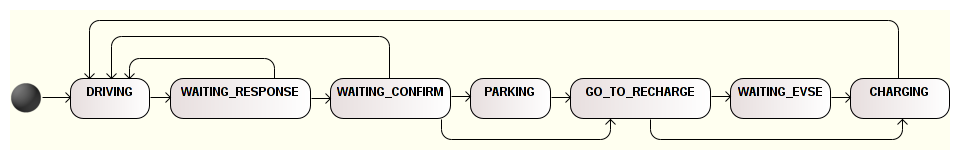
\includegraphics[width=1.0\textwidth]{assets/car-fsmd.png}
	\caption{Automa a stati finiti di descrizione del veicolo.}
	\label{fig:car-fsmd}
\end{figure}

Al termine del ciclo di vita del modulo si provvede all'eliminazione dei dati relativi al veicolo dal SIB.

\subsection{Battery}\label{sec:battery}

Il modulo fornisce il modello di consumo energetico del veicolo. Non è esatto parlare di modello della batteria dal momento che le equazioni usate sono relative al lavoro e non strettamente legate all'elettrotecnica poiché troppo complesse da simulare. Il modello implementato rimane abbastanza fedele alla realtà in virtù del fatto che è stato validato con dati sperimentali raccolti durante la visita al CRF.

Determinante al fine di modellare e validare il consumo è stato il lavoro di Alfredo D'Elia prima e Marco di Nicola (\cite{dinicola2014}) dopo. Il modello attualmente tiene conto della pendenza della strada grazie alla quale si può calcolare l'energia richiesta in salita e quella guadagnata in discesa. A questo si aggiunge la ricarica dovuta alla frenata rigenerativa.

Il ciclo di vita del modulo batteria è determinato dall'auto-invio di messaggi la cui schedulazione è indipendente da quella del modulo \code{CarLogic}.

Il modulo \code{Battery} può assumere due stati: \code{CHARGING} e \code{DISCHARGING}, definiti nell'enumerazione \code{BatteryState}. Le relative funzioni handler sono \code{handleDischarge} e \code{handleCharge}. Lo stato della batteria viene modificato da \code{CarLogic}. Giunti a una colonnina viene impostato lo stato \code{CHARGING}. Si passa inoltre a \code{Battery} un riferimento all'EVSE corrispondente il quale fornisce le informazioni sulla potenza della colonnina e quindi il tempo necessario alla ricarica, terminata la quale \code{CarLogic} imposta lo stato del modulo batteria in \code{DISCHARGING} e dirige il veicolo verso una destinazione casuale.

Il modulo \code{Battery} ha anche la funzione di eliminare il veicolo dalla simulazione quando termina la carica della batteria.

\subsubsection{I parametri}

Elenco nel seguito i parametri che caratterizzano il modulo batteria. I valori di default sono relativi al Fiat Daily fornito dal CRF in quanto disponendo dei dati sperimentali abbaiamo potuto validare al meglio per confronto quelli generati dalle simulazione.

\begin{itemize}
	\item \textbf{manufacturer}: costruttore della batteria impostato di default a ``Simens'' in quanto partner del progetto IoE;
	\item \textbf{engineEfficense}: efficienza della gestione energetica del motore. Varia tra 0 e 1.
	\item \textbf{socPerc}: carica iniziale del veicolo (State Of Charge). Varia da 0 a 1, dove 1 indica una quantità di carica pari alla capacità della batteria;
    \item \textbf{capacity}: capacità della batteria misurata in Kilowattora (kWh);
    \item \textbf{maxVoltage}: voltaggio massimo erogato misurato in Volt (V);
    \item \textbf{voltage}: voltaggio corrente di erogazione in Volt (V);
    \item \textbf{stateOfHealth}: stato di vita della batteria. Varia tra 0 e 1. Attualmente non è considerato nel modello;
    \item \textbf{maxCurrentIn}: massima intensità di corrente in entrata misurata in Ampere (A);
    \item \textbf{maxCurrentOut}: massima intensità di corrente in uscita misurata in Ampere (A);
    \item \textbf{nominalTempearture}: massima temperatura a cui può lavorare il motore misurata in Gradi Celsius (\textcelsius). Attualmente non è considerata nel modello.
    \item \textbf{recordVectors}: indica se registrare o meno le statistiche sulla batteria. Questi dati tendono a far crescere molto la dimensione dei file che li contengono;
    \item \textbf{regenerativeBrakingEfficiency}: efficienza della frenata rigenerativa;
\end{itemize}

\subsubsection{Consumo del veicolo}

Il modello di consumo è implementato nella funzione \code{handleDischarge()}. I dati necessari al calcolo sono: 

\begin{itemize}
	\item \textbf{Velocità attuale}: fornita da Veins che ne tiene bufferizzato il valore senza eseguire comandi tramite TraCI. A volte, a veicolo fermo, Veins ricorda erroneamente il valore della velocità precedente la fermata provocando un consumo della batteria anche a veicolo parcheggiato. Risulta quindi necessario verificare manualmente che il veicolo non sia parcheggiato.
	\item \textbf{Accelerazione}: poiché non è fornita da TraCI occorre calcolarla come differenza tra la velocità attuale e quella registrata nell'ultima chiamata a \code{handleDischarge()} rapportata al tempo simulato trascorso.
	\item \textbf{Angolo di inclinazione stradale}: indicato con $\alpha$ è fornito dalla funzione \code{getInclinationRad()} che lo ricava a partire da 2 punti nel piano tridimensionale determinata dalla funzione \code{getLatLonAlt()} di \code{CarLogic} mediante una doppia chiamata a SUMO. La prima necessaria ad ottenere la posizione sulla strada corrente, la seconda per effettuare la sua conversione in latitudine, longitudine, altitudine. Fortuna vuole che questa feature sia stata recentemente introdotta in SUMO.
	\item \textbf{La quantità di carica}: poiché i calcoli successivi restituiscono valori in kWh occorre convertire la quantità di carica espressa in percentuale (socPerc) in kWh con la formula: $soc_{kWh} = soc_{\%} \cdot capacity$.
\end{itemize}

Le funzioni necessarie a calcolare distanza e inclinazione a partire da punti in 3 dimensioni sono state parzialmente ereditate dalla libreria UniboGeoTools e si trovano nel file \code{Util.cc}. Si noti che la distanza viene calcolata attraverso applicazione di proiezione ortogonale (\code{getEquirectangular ApproximationDistance()}) che non è la formula più precisa per la distanza tra due punti espressi in coordinate latitudine/longitudine a causa della curvatura terrestre. Ma viste le brevi distanze in gioco quindi ridotto l'errore che ne deriva, la maggiore velocità di esecuzione ha determinato la scelta del suo utilizzo al posto di formule più precise come la formula dell'emisenoverso, più onerosa in termini di performance.

Nello spostamento del veicolo sono considerate tre forme diverse di dispendio energetico :

\begin{itemize}
	\item \textbf{$L_m$}: lavoro compiuto dal motore per far muovere il veicolo.
	\item \textbf{$L_g$}: lavoro necessario a superare l'attrito delle gomme sull'asfalto.
	\item \textbf{$L_a$}: lavoro necessario a superare la resistenza dell'aria.
\end{itemize}

\noindent
Considerando:

\begin{center}
	$\boxed{m \cdot a = F - m \cdot g \cdot \sin{\alpha} }$
\end{center}
~
\noindent
La forza necessaria a spostare il veicolo tenendo conto della pendenza è:

\begin{center}
	$\boxed{F = m \cdot (a + g) \cdot \sin{\alpha} }$
\end{center}

\noindent
Ne segue che il lavoro necessario a spostare il veicolo è:

\begin{center}
	$\boxed{L_m = \frac{1}{engineEfficiency} \cdot \Delta t \cdot F \cdot \frac{V + V_{old}}{2}}$
\end{center}

\noindent
La massa del veicolo ($m$) è fornita dai parametri del modulo \code{CarLogic} precedentemente introdotti. L'efficienza del motore è definita tra i parametri del modulo \code{Battery}.
\\\\
Il lavoro $L_g$ per vincere l'attrito delle gomme sull'asfalto è dato da:

\begin{center}
$\boxed{L_g = \frac{1}{engineEfficiency} \cdot \Delta t \cdot (m \cdot g \cdot \cos{\alpha} \cdot cRoll) \cdot \frac{V + V_{old}}{2}}$
\end{center}
\noindent
dove $cRoll$, introdotto in \code{CarLogic}, è l'attrito delle gomme sull'asfalto.
\\\\
\noindent
Infine il lavoro necessario a vincere la resistenza dell'aria è:

\begin{center}
	$\boxed{L_a = \frac{1}{engineEfficiency} \cdot \Delta t \cdot \frac{(\rho_{air} \cdot cDrag \cdot across)}{2} \cdot 	(\frac{V + V_{old}}{2})^3}$
\end{center}

Ne consegue che il consumo energetico totale, espresso in kWh è dato da:

\begin{center}
	$\boxed{energyConsumption = \frac{L_m + L_g + L_a}{3600000}}$
\end{center}
\noindent
che viene sottratto alla quantità di carica in kWh precedentemente calcolata che viene ritrasformata in percentuale.

\subsubsection{Frenata Rigenerativa}

Il freno rigenerativo è un particolare tipo di freno che recupera energia utile estraendola da una quota di quella che normalmente si dissipa in aria sotto forma di calore durante il rallentamento del veicolo (diminuzione di energia cinetica). Nel nostro sistema la frenata è determinata da accelerazione negativa. In questo caso $L_m$, che contribuirebbe all'energia consumata dal veicolo, non viene considerato e al suo posto viene considerata l'energia cinetica prodotta nella decelerazione del veicolo in Joule (J):

\begin{center}
	$\boxed{E_{kin} = \frac{1}{2} \cdot m \cdot (V^2 - V_{old}^2) \cdot \eta_{rig}}$
\end{center}

Dove $\eta_{rig}$ è la percentuale di energia recuperabile da quella prodotta rappresentata con il parametro di \code{Battery}: \code{regenerativeBrakingEfficiency}. Questo dipende dall'efficienza del meccanismo di frenata/rigenerazione che ha un un limite teorico del 30\% (valore di default) prodotto da recenti studi del IDSC (Institute for Dynamic Systems and Control) svizzero.

Determinante per il raggiungimento di questo risultato è stato il contributo di Marco Di Nicola.

\subsubsection{Ricarica del veicolo}

Il modello di ricarica è implementato nella funzione \code{handleCharge()}. Per determinare la carica è necessario disporre delle informazioni sull'EVSE al quale si è allacciati. Un'istanza di un oggetto che rappresenta l'EVSE viene passata al modulo \code{Battery} dal modulo \code{CarLogic}.

Viene presa la potenza della colonnina espressa in kW  ($power_{kW}$) e a ogni iterazione il guadagno energetico viene cosi calcolato:

\begin{center}
	$\boxed{soc_{kWh} =  soc_{kWh} + (power_{Kw} \cdot \Delta t) \cdot 3600}$
\end{center}

\noindent
Quando la carica raggiunge la capacità della batteria il processo viene interrotto e il veicolo lascia la colonnina.

\subsection{DriverBeahviour}

Il modulo si occupa di modellare alcuni comportamenti dell'autista del veicolo. Attualmente non è particolarmente evoluto in quanto, essendo stato introdotto successivamente \code{CarLogic}, parte della logica è implementata in quest'ultimo.

\subsubsection{I parametri}

I parametri di questo modulo consistono in coefficienti statistici che determina la propensione verso un comportamento.

\begin{itemize}
	\item \textbf{parkingProbabilitWaitingNoRes}: determina la probabilità di fermarsi ad attendere presso una colonnina che il veicolo attualmente in carica finisca.
	\item \textbf{parkingProbabilitWaitingRes}: 
	\item \textbf{maxWaitingTime}
	\item \textbf{minWaitingTime}
	\item \textbf{chooseTheNearest}
\end{itemize}



\section{Implementazione}

Esisteva già una versione del simulatore ma era a puro titolo dimostrativo e di demo e soffriva del fatto che era stato sviluppato da diverse persone (me compreso) in tempi molto brevi e con deadline che corrispondendo a demo internazionali si era costretti a rispettare. Questo ha portato ad avere un codice farraginoso e pieno di memory leak. Basti pensare che la prima versione del simulatore allocava RAM esponenzialmente e già dopo 2000 secondi si poteva arrivare ad avere un occupazione di 4GB.

La prima cosa che ho fatto, quando ho capito che la situazione stava diventando ingestibile è stato profilare e rifattorizzare il codice. La profilazione è avvenuta tramite il tool Valgrind grazie al quale sono riuscito ad ottenere un cosumo di memoria lineare, infatti, dove prima venivano occupati 4GB, sono riuscito a raggiungere il traguardo dei 100MB. La rifattorizzazione del codice invece è stata più complessa in quanto diverse mani hanno messo mano con diversi stili di programmazione. 

\subsection{Logging}

\subsection{SibController}

\subsection{GcpController}

\subsubsection{GCP e EVSE}

\subsection{Utility}

\section{L'ambiente di simulazione}

In questa sezione verranno descritti in dettaglio i componenti necessari a creare un ambiente di simulazione funzionante.

La logica del simulatore è implementata attraverso moduli di OMNeT++. Grazie ad essi sono implementati, i modelli di consumo dei veicoli elettrici, i comportamenti degli degli autisti e la rete di distribuzione elettrica cittadina. L'unico aspetto non implementato è la guida dei veicoli in quanto è gestita da SUMO.

I file di configurazione di SUMO sono generati da script che in base ai parametri specificati possono variare l'intensità del traffico.


\subsection{Generazione file di Configurazione}

Dopo aver scaricato compilato ed installato tutti i componenti è necessario generare i file di configurazione riguardanti lo scenario che si vuole simulare. 

\subsection{Download Scenario}

A questo punto è necessario scegliere quale scenario si vuole simulare. Lo scenario di Bologna è già disponibile nella cartella \code{simulator/veins-2.1/examples/veins/bologna} siccome è quello di nostro interesse.

Nel caso in cui si sia interessati ad uno scenario diverso da quello di Bologna il modo più semplice per ottenere la mappa desiderata è andare all'indirizzo \url{http://www.openstreetmap.org/export} e scaricarsi l'area interessata. La dimensione delle mappe scaricabili è limitata onde evitare la saturazione della banda del server. Per sopperire a questa mancanza SUMO mette a disposizione un tool situato in \code{<SUMO_HOME>/tools/import/osm/osmGet.py} che permette di scaricare mappe di dimensione arbitraria. Per l'utilizzo di questo tool rimando alla documentazione dello script oppure alla pagine ufficiale:

\url{http://sumo-sim.org/userdoc/Networks/Import/OpenStreetMapDownload.html}.

\subsubsection{Profilo Altimetrico}\label{profilo-altimetrico}

Da notare che le mappe di Open Street Map non contengono le informazioni relative al profilo altimetrico. È quindi necessario "arricchire" la mappa scaricata con tali informazioni. Il programma utilizzato a questo scopo è Osmosis, presente nella cartella \code{osmosis} del progetto. In particolare ho usato \code{osmosis-srtm-plugin_1.1.0} che permette, attraverso l'interrogazione di file SRTM (scaricabili da \url{http://dds.cr.usgs.gov/srtm/version2_1/SRTM3/}, di inserire i dati del profilo altimetrico nelle mappe di Open Street Map. 

Di seguito viene mostrato l'utilizzo del Osmosis e del relativo plugin considerando \code{\$SRTM_HOME} la cartelle che contiene i file SRTM e \code{\$CITY_NAME} il nome della città. Quindi avendo, ad esempio, \code{bologna.osm}, ovvero la mappa della città di Bologna senza dati riguardanti il profilo altimetrico, in output avremo \code{bologna_srtm.osm}, ovvero la stessa mappa con i dati estratti dai file SRTM.

\begin{bash}
osmosis -plugin org.srtmplugin.osm.osmosis.SrtmPlugin_loader --read-xml "\$CITY_NAME".osm --write-srtm locDir="\$SRTM_HOME" locOnly=true repExisting=false --write-xml "\$CITY_NAME"_srtm.osm
\end{bash}

%

Da tenere in considerazione il fatto che il comando mostrato è incluso nello script di generazione automatica da me creato al fine di velocizzare la configurazione dello scenario.

\subsection{Generazione XML di SUMO}

SUMO necessita di file di configurazione in XML che descrivono la rete stradale, i poligoni dei palazzi e i percorsi di ogni singolo veicolo. Siccome ognuno di questi file, per essere generato, richiede un apposito comando il quale a sua volta richiede vari parametri, ho creato uno script che data la mappa di una città in formato Open Street Map esegue tutte le operazioni necessarie.

Verranno comunque analizzati tutti i comandi singolarmente in modo d aavere una panoramica sulle scelte implementative.

\subsubsection{La rete Stradale (.net.xml)}

Il file della rete stradale viene generato attraverso il tool \code{netconvert} direttamente dalla mappa di Open Stree Map. Oltre al file \code{.osm} è necessario anche un file di supporto che istruisca SUMO sui vincoli e i limiti di velocità delle strade importate. Noi ne utilizziamo uno creato ad hoc per il traffico tedesco. 

Qui sotto ne riporto un frammento a puro titolo esemplificativo, il file intero si trova in \code{simulator/veins-2.1/examples/veins/bologna/osm-urban-de.typ.xml}

\begin{xml}
<types xmlns:xsi="http://www.w3.org/2001/XMLSchema-instance">
  <type id="highway.motorway" priority="13" numLanes="2" speed="41.667"
                oneway="true" disallow="bicycle pedestrian"/>
  <type id="highway.motorway_link" priority="8" numLanes="1" speed="13.889"/>
  <type id="highway.trunk" priority="12" numLanes="2" speed="13.889"/>
  <type id="highway.trunk_link" priority="8" numLanes="1" speed="13.889"/>
  <type id="highway.primary" priority="11" numLanes="2" speed="13.889"/>
  <type id="highway.primary_link" priority="8" numLanes="1" speed="13.889"/>
  <type id="highway.secondary" priority="10" numLanes="2" speed="13.889"/>
  ....
</types> 
\end{xml}

Di seguito passiamo ad un analisi dettagliata di tutti i parametri passati a \code{netconvert}:

\begin{itemize}
	\item \textbf{-{}-type-files}: Specifica il file che contiene i vincoli e i limiti, quello citato sopra.
	\item \textbf{-{}-ramps.guess}: Prova a capire dove sono le rampe e ad eseguirne l'importazione
	\item \textbf{-{}-remove-edges.by-vclass}: Siccome Open Street Map include un infinità informazioni del tutto inutili al nostro fine (ferrovie, piste ciclabili, aree pedonali ecc..) con questo parametro si indicano le classi da non importare (\code{bicycle,pedestrian...})
	\item \textbf{-{}-geometry.remove}:
	\item \textbf{-{}-remove-edges.isolated}:
	\item \textbf{-{}-tls.join}:
	\item \textbf{-{}-osm-files}:
	\item \textbf{-{}-output.street-names}:
	\item \textbf{-{}-output.original-names}:
	\item \textbf{-{}-output-file}:
\end{itemize}

Siccome Open Street Map include molte informazioni che sono del tutto inutili al nostro fine (ferrovie, piste ciclabili, aree pedonali ecc..) bisogna istruire \code{netconvert} affinché le escluda dall'importazione. 

%\begin{bash}
%netconvert --type-files osm-urban-de.typ.xml --ramps.guess --remove-edges.by-vclass hov,taxi,bus,delivery,transport,lightrail,cityrail,rail_slow, rail_fast,motorcycle,bicycle,pedestrian --geometry.remove --remove-edges.isolated true --tls.join --osm-files "$MAP_FILE" --output.street-names --output.original-names --output-file "$CITY_NAME".net.xml
%\end{bash}

